\documentclass{article}
\usepackage[colorlinks = true,
            linkcolor = blue,
            urlcolor  = blue,
            citecolor = blue,
            anchorcolor = blue]{hyperref}
\usepackage{graphicx}
\usepackage[parfill]{parskip}
\usepackage[margin=1in]{geometry}
\usepackage{titling}

\graphicspath{{images/}}
\pagenumbering{gobble}
\title{Raytracing Project}
\author{Jared Givens, Ahbi Sohal, Noah Krim}
\date{28 May, 2023}

\pretitle{% add some rules
  \begin{flushleft}
    \Large
    \bfseries
    % \Huge\bfseries
}%, make the fonts bigger, make the title (only) bold
\posttitle{%
  \end{flushleft}%
}
\preauthor{%
  \begin{flushleft}
    \begin{tabular}[t]{@{}l@{}}%
}
\postauthor{%
    \end{tabular}
  \end{flushleft}%
}
\predate{%
  \begin{flushleft}
}
\postdate{%
  \end{flushleft}%
}


\begin{document}
\maketitle

\large
Description

\normalsize
The program outputs color values of pixels with raytracing techniques. 
It begins by initalizing virtual geometry and a camera. Then it sends rays from the camera 
into the virtual space. 

For each pixel a series of uniformly random rays are 
cast to gather a color value. the color values are then averaged to achive anti 
aliassing. 

Each ray iterates over the scenes geometry to determine the nearest 
intersection. The nearest intersection's color is then multiplied against the 
rays running total color value. The ray then reflects and scatters or refracts 
based on the properties of the material that was intersected. The process of 
accumulating color and bouncing continues until the ray fails to collide with 
an object or reaches the maximum ray depth. If the ray fails to collide, the 
program adds the contribution of the skybox to complete the color.  
If the ray reaches the 
maximum bounce depth the color is set to black.  

\large
Justification

\normalsize
Our serial prototype was only capable of outputing a single frame in 5.971 seconds
(wall-clock time 2020 Macboock 2 GHz 16 GB). This program is an excellent 
candidate for CUDA, because the code of each ray can run in parallel. One of the 
biggest difficulties partitioning the geometry to be intersected. 
The 
majoraty of the time is spent computing the ray intersections and bounces which 
have no data dependencies. Additionally the majoraty of code is linear algebra 
with a few branches that could be removed with better equations. 

\large
Qualification

\normalsize
Our team can complete this project because we completed a 
\href{https://github.com/JaredGivens/ECS158-Raytracing}{serial prototype}.
We followed the tutorial
\href{https://raytracing.github.io/books/RayTracingInOneWeekend.html}{Ray Tracing In OneWeekend}
the program writes a ppm to stdout which can be converted to a PNG.
If time permits we have plans to trying to integrate OpenGL BVH, triangles, model loading, lights
and textures.
The project uses CMake to create the makefile.
to create the makefile.



Here is a frame from the serial output:

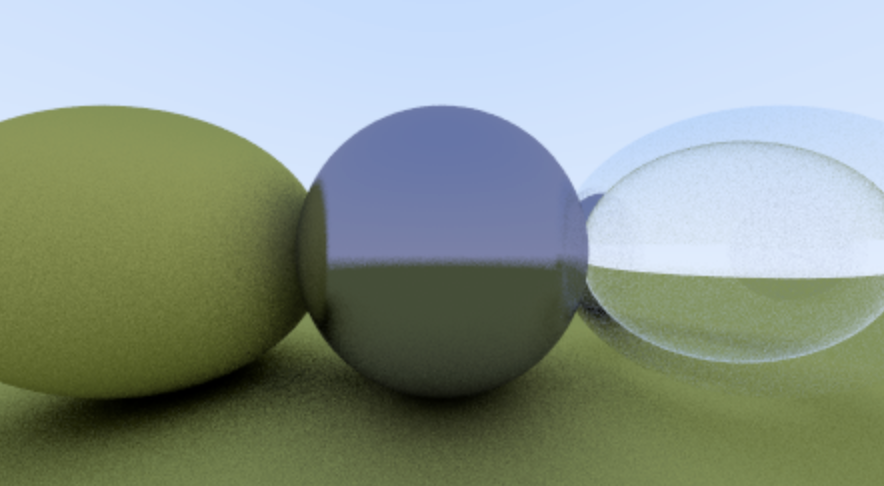
\includegraphics[scale=0.5]{rtsc}

\end{document}.